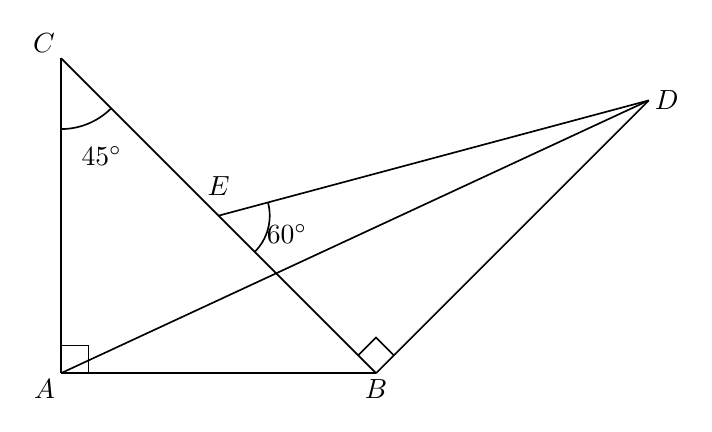
\begin{tikzpicture}[x=1cm,y=1cm,font=\normalsize,
 geometry edge/.style={solid,line width=.6pt},
 geometry mark/.style={solid,line width=.6pt},
 geometry label/.style={font=\normalsize,inner sep=2pt}]
\coordinate (A) at (0.000000,0.000000);
\coordinate (B) at (4.000000,0.000000);
\coordinate (C) at (0.000000,4.000000);
\coordinate (E) at (2.000000,2.000000);
\coordinate (D) at (7.464102,3.464102);
\draw[geometry edge] (A)--(B);
\draw[geometry edge] (A)--(C);
\draw[geometry edge] (C)--(E);
\draw[geometry edge] (E)--(B);
\draw[geometry edge] (B)--(D);
\draw[geometry edge] (E)--(D);
\draw[geometry edge] (A)--(D);
\draw[geometry mark] (0.350000,0.000000)--(0.350000,0.350000)--(0.000000,0.350000);
\draw[geometry mark] (3.773726,0.226274)--(4.000000,0.452548)--(4.226274,0.226274);
\draw[geometry mark] (0.000000,3.100000) arc (-90:-45:0.900000);
\draw[geometry mark] (2.459619,1.540381) arc (-45:15:0.650000);
\node[font=\normalsize] at (0.516622,2.752762) {$45^\circ$};
\node[font=\normalsize] at (2.869333,1.767062) {$60^\circ$};
\node[geometry label,below left] at (A) {$A$};
\node[geometry label,below] at (B) {$B$};
\node[geometry label,above left] at (C) {$C$};
\node[geometry label,right] at (D) {$D$};
\node[geometry label,above=5pt] at (E) {$E$};
\end{tikzpicture}
